% ==================================================
% ==================================================
\chapter{Methods}
\label{methods}
This chapter describes the methods used in our experiments. In section~\ref{methods:models}, we start by defining the problem~\ref{methods:models:problem-definition}, then we present one simple approach to decode images using linear regression and four more advanced ones which use neural networks, some of which are inspired by~\citep{zhang2020reconstruction}. We use the model from this paper, along with the linear regression, as a baseline comparison.

In the following section~\ref{methods:losses}, we present several loss functions that we use for training and testing the model performance. We use simple ones like $L_1$ ~\ref{methods:losses:L1} or MSE ~\ref{methods:losses:MSE}, as well as a more complex one implemented through the use of another neural network ~\ref{methods:losses:adversarial}.

The details about the software and packages we used are in the last section~\ref{methods:implementation-details}.

The experiments using these models and these losses are described in the subsequent chapter~\ref{experiments}.

% ==================================================
\section{Models}
\label{methods:models}
To address the problem of decoding visual stimuli, we implemented several different models. Some were selected as a simple baseline~\ref{methods:models:linear-regression}, and others were based on state-of-the-art CNN networks~\ref{methods:models:CNNv4} for image decoding~\citep{zhang2020reconstruction}. The ones that performed the best are presented in this section. We start this section by properly defining the problem we are solving~\ref{methods:models:problem-definition}.


% **************************************************
\subsection{Problem Definition}
\label{methods:models:problem-definition}
The problem of decoding image stimuli from cortical activity in this thesis is defined as follows. The cortical activity consists of the responses of the neurons in the primary visual cortex to visual stimuli. The goal of the decoding process is to accurately generate a visual stimulus image that is similar to the one presented to the subject based on the recorded cortical activity.

Let us assume that we are provided with a cortical activity encoded as $\#{x} \in \SX$ where $\SX = \mathbb{R}^{n}$ denotes the space of all possible cortical activity encodings using $n$ neurons.
We are trying to predict stimuli $\#{s} \in \SY$, where $\SY = [0;1]^{h \times w}$ denotes space of all possible stimuli images of width $w$ and height $h$. The stimuli images are therefore grayscale and the pixel values are in the range [0;1], where 0 is the darkest and 1 is the lightest value. In our settings, we can assume $w=h$.

The goal is to create a generator $g:\ \SX \rightarrow \SY$ from a space of all such functions $\SG$ which for given cortical activity vector $\#{x} \in \SX$ predicts a decoded stimulus image $\#{s} \in \SY$. Let us first define
\begin{equation}
\label{equation:predictor-loss}
l(\#{s}, g, \#{x}) = \SL(\#{s}, g(\#{x} ; \#\theta))\:,
\end{equation}
% \begin{equation}
% \label{equation:predictor-loss-mean}
% \SL(\#{s}, g(\#{x} ; \#\theta)) = \sum_{i=1, j=1}^{w, h}{\SL_{i,j}(s_{i,j}, g_{i,j}(\#{x} ; \#\theta))} \cdot \frac{1}{w+h}\:,
% \end{equation}
% where $\SL(\#{s}, g(\#{x} ; \#\theta))$ resp. $\SL_{i,j}(s_{i,j})$ is an arbitrary differentiable loss function (image-wise resp. point-wise defined) (find more details about used loss functions in section~\ref{methods:losses}) which given the stimulus $\#{s} \in \SY$ and generated image given by the generator function $g$ returns the loss value. Values $\#\theta$ are the parameters of the generator function. By $f_{i,j}$ we denote pixel value on $i$-th column and $j$-th row of function $f$.

% Due to minimization, we can simplify the formula~\ref{equation:predictor-loss-mean}, we can also omit the parameters of function $g$ for brevity
% \begin{equation}
% \label{equation:simplified-loss}
% \SL(\#{s}, g) = \sum_{i=1, j=1}^{w, h}{\SL_{i,j}(s_{i,j}, g_{i,j})}\:.
% \end{equation}
where $\SL(\#{s}, g(\#{x} ; \#\theta))$ is an arbitrary differentiable loss function (find more details about used loss functions in section~\ref{methods:losses}). Values $\#\theta$ are the parameters of the generator function.


We want such $g \in \SG$, lets denote it $g^* \in \SG$, that minimizes the value $l(\#{s},g,\#{x})$:

\begin{equation}
%\label{equation:predictor}
% l_{min}(\#{x}) = \argmin_{\#{s}\in \SY, g\in \SG}{l(\#{s},g,\#{x})}\:,
\argmin_{\#{s}\in \SY}l(\#{s},g^*,\#{x}) = \argmin_{\#{s}\in \SY, g\in \SG}{l(\#{s},g,\#{x})}\:.
\end{equation}
%  $g^*$ satisfies
% \begin{equation}
% %\label{equation:predictor-loss-mean}
% \argmin_{\#{s}\in \SY}l(\#{s},g^*,\#{x}) = l_{min}(\#{x})\:.
% \end{equation}


We present several CNN models in the following sections to find $g^*$ using only the standard CNN layers -- namely convolutional layers, fully connected layers, convolutional transpose layers, and batch normalization layers. The CNN models use standard ReLU activation function internally and utilize a sigmoid activation function in the final layer, resulting in the output values being constrained within the range of [0, 1], which matches the range of the stimuli images.

We learn the model parameters, and therefore train the model to approximate $g^*$, by minimizing the formula
\begin{equation}
\label{equation:predictor-loss-minimization}
L(\#\theta) = \sum_{j=1}^m{\SL(\#{s}, g(\#{x} ; \#{\theta}))}\:,
\end{equation}
where $\{(\#{x}^j, \#{s}^j) \in (\SX \times \SY) \mid j=1,2,\dots,m\}$ is the training dataset with $m$ training samples.


% **************************************************
\subsection{Linear Regression}
\label{methods:models:linear-regression}
As a simple baseline, linear regression was used based on its deterministic properties to always converge to the same optimum value. The goal of linear regression is to find a linear relationship that best fits the given data.

In simple linear regression, the relationship between the dependent variable Y and the independent variable X is modeled as a straight line. The equation of the line can be written as:

\begin{equation}
Y = \beta_0 + \beta_1 X + \epsilon
\end{equation}

where $\beta_0$ is the intercept, $\beta_1$ is the slope, and $\epsilon$ is the error term which represents the unexplained variability in the data.

The objective of linear regression is to estimate the values of the parameters $\beta_0$ and $\beta_1$ that best fit the data. This is typically done using the method of least squares, which involves minimizing the sum of the squared errors:

\begin{equation}
\sum_{i=1}^{n}(Y_i - \beta_0 - \beta_1 X_i)^2
\end{equation}

where $n$ is the number of observations.

In our case, to be able to use this method, we linearize the stimuli images $\#{s} \in \SY$ from 2D matrices $w \times h$ to vectors of size $w * h$.


% **************************************************
\subsection{CNNv1}
\label{methods:models:CNNv1}
The first neural network presented is a CNN model that generates an image on the latest layer. 

It has a sequential architecture with several transposed convolutional layers with increasing numbers of filters. Each transposed convolutional layer is followed by a batch normalization layer and a ReLU activation function. The final layer is a transposed convolutional layer with a sigmoid activation function that outputs the reconstructed image.

The network has a total of 278,197,825 parameters, all of which are trainable. The architecture is graphically presented on the picture~\ref{img:methods:models:CNNv1}. Since the output is not 110x110px, we use bilinear interpolation to create the proper output size.

\begin{figure}[H]\centering
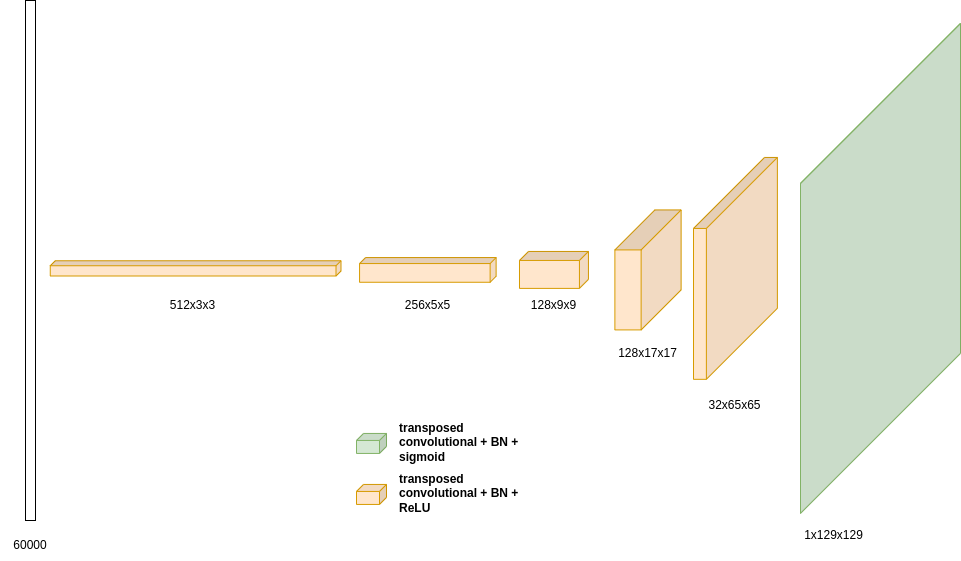
\includegraphics[width=140mm]{img/cnnv1.drawio.png}
\caption{First version of the CNN architecture simply takes the input and uses only transpose convolutional layers without any linear layers to produce the output.}
\label{img:methods:models:CNNv1}
\end{figure}


% **************************************************
\subsection{CNNv2}
\label{methods:models:CNNv2}
The second model is a CNN-based model with a total of 2 sequential parts.

The first part is a fully connected layer consisting of a linear transformation followed by batch normalization, ReLU activation, and dropout. The second part is a sequence of 6 transpose convolutional layers, also known as deconvolutional layers, followed by batch normalization and ReLU activation, and the final layer is a sigmoid activation function. 

The second part of the model takes an input tensor of size [B, 64, 8, 8] and outputs a tensor of size [B, 1, 289, 289], where $B$ is the batch size. The model has a total of 34,695,873 trainable parameters. Since the output is not 110x110px, we again use the same approach by adding bilinear interpolation to create the required output size. The architecture is drawn on picture~\ref{img:methods:models:CNNv2}.

\begin{figure}[H]\centering
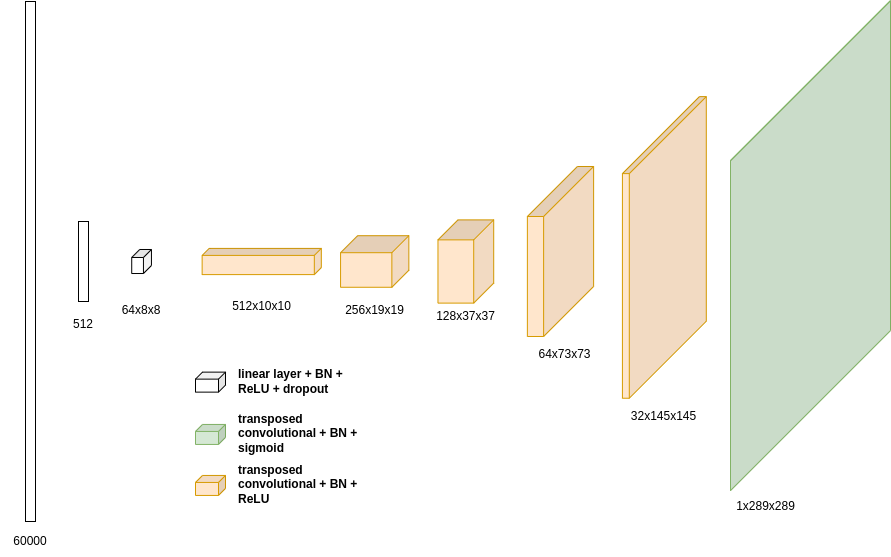
\includegraphics[width=140mm]{img/cnnv2.drawio.png}
\caption{Second version of the CNN architecture. This architecture contains a linear-encoding part and a decoding part producing the final output.}
\label{img:methods:models:CNNv2}
\end{figure}


% **************************************************
\subsection{CNNv3}
\label{methods:models:CNNv3}
The third generative model designed to produce images consists of two main components: a fully connected neural network and a convolutional neural network.

The fully connected network takes a cortical activity vector as input and outputs a 12100-dimensional feature vector. The feature vector is then reshaped into a 110x110px intermediate image tensor and passed through a series of transposed convolutional layers. These layers preserve the spatial dimensions and gradually decrease the channel resolution of the tensor until it has the same dimensions as the desired output image. 

The final layer of the convolutional neural network is a sigmoid activation function that squashes the pixel values of the output image to the range [0, 1]. This property is consistent across all of our models. This model has 38,527,629 trainable parameters and generates images with a size of 110x110 pixels exactly. This architecture is shown in picture~\ref{img:methods:models:CNNv3}.

\begin{figure}[H]\centering
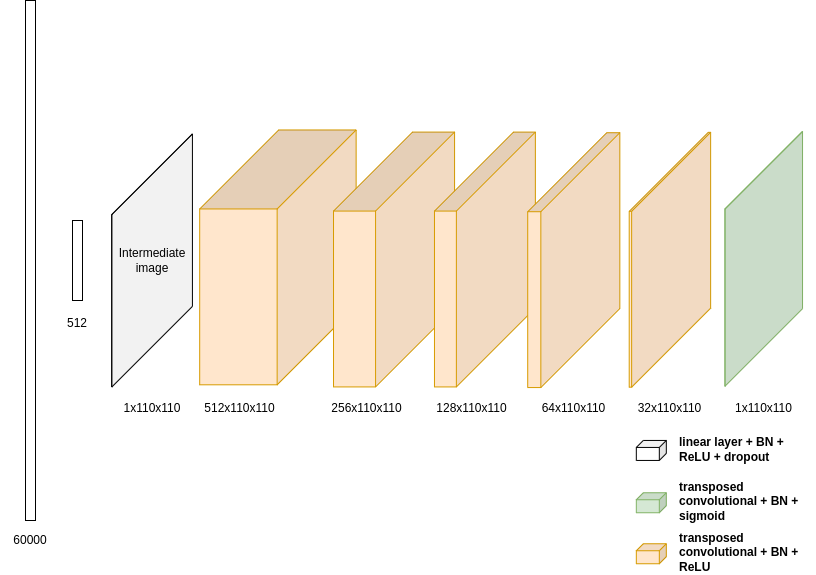
\includegraphics[width=140mm]{img/cnnv3.drawio.png}
\caption{Third version of the CNN architecture. Since the creation of the intermediate image, the dimensions stay the same except for the number of channels.}
\label{img:methods:models:CNNv3}
\end{figure}


% **************************************************
\subsection{CNNv4}
\label{methods:models:CNNv4}
This is a fourth CNN model for image generation, it is an implementation from paper~\citep{zhang2020reconstruction}\footnote{A detailed implementation code in Keras is available at \url{https://github.com/jiankliu/Spike-Image-Decoder/blob/main/SID.py}}. It consists of three sequential blocks. The first block is a fully connected neural network with two linear layers, batch normalization, ReLU activation, and dropout. This produces an intermediate image of size 110x110 pixels with a sigmoid activation function. The second block is a convolutional neural network with four convolutional layers, batch normalization, ReLU activation, and dropout. The third block is an upsampling neural network with four upsampling layers, four convolutional layers, batch normalization, ReLU activation, and dropout.

The input to this model is again a vector of cortical activity, and the output is an image of size 110x110 with each pixel between values 0 and 1. The model is using the sigmoid function as the final activation function to produce the output image. This architecture is drawn on picture~\ref{img:methods:models:CNNv4}.

The model has a total of 37,107,157 parameters out of which 30,720,512 parameters are contained in the first block containing linear layers.

\begin{figure}[H]\centering
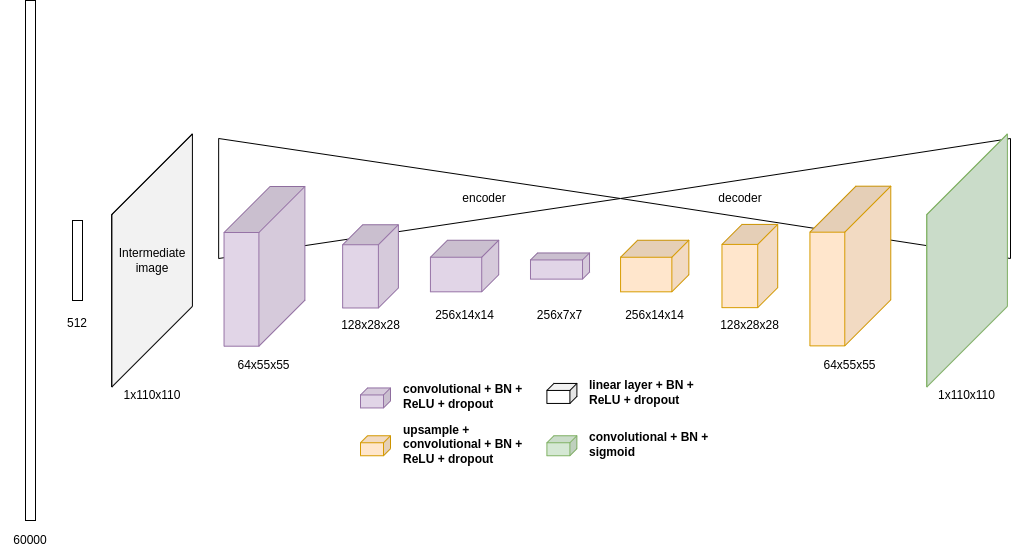
\includegraphics[width=140mm]{img/cnnv4.drawio.png}
\caption{Fourth version of the CNN architecture. The first part producing the intermediate image is here easily distinguishable from the encoder-decoder part of the architecture.}
\label{img:methods:models:CNNv4}
\end{figure}




% ==================================================
\section{Losses}
\label{methods:losses}
To train the generator function~\ref{equation:predictor-loss-minimization}, we tried several loss functions $\SL$ that are commonly used for image restoration~\citep{zhao2016loss}. It is not clear which one is optimal: since the resulting image will be evaluated by a human observer, as we need to use perceptually motivated losses. Sometimes, multiple loss functions are combined to produce a more sophisticated one~\citep{zhao2016loss}. In our experiments, the loss functions are used both for training and evaluation as \textit{accuracy} metrics.


% **************************************************
\subsection{L1}
\label{methods:losses:L1}

$L_1$ loss, also known as the mean absolute error (MAE), is a measure of the difference between two continuous variables. This loss function can be used in regression analysis to evaluate the accuracy of a predictive model.

The $L_1$ loss of the predicted value $\hat{y}$ and the true value $y$ is defined as:

\begin{equation}
L_1(\hat{y},y) = |\hat{y} - y|\:.
\end{equation}

The $L_1$ loss is a pixel-wise loss that computes the absolute difference between predicted and true values, which is then averaged across pixels.  It has the property of being robust to outliers, as the loss is not affected by large differences between the predicted and true values. The interpretability of this loss function is especially evident when compared with other loss functions that we use.


% **************************************************
\subsection{MSE}
\label{methods:losses:MSE}
Mean squared error (MSE) is a loss function used in regression analysis to evaluate the accuracy of a model. It measures the average squared difference between the predicted and true values.

The MSE between the predicted value $\hat{y}$ and the true value $y$ is defined as:

\begin{equation}
MSE(\hat{y},y) = (\hat{y} - y)^2\:.
\end{equation}

The squared difference between the predicted and true values penalizes large errors more than small errors. It is another possible choice for regression problems where the goal is to minimize the average squared difference between the predicted and true real values. This loss function is computed pixel-wise and then averaged across all the pixels.


% **************************************************
\subsection{SSIM}
\label{methods:losses:SSIM}
The structural similarity (SSIM) index is a popular loss function used in image processing to measure the similarity between two images. It compares the structural information of the images, including luminance, contrast, and structure. The first definition was presented in~\citep{wang2004image}.

The SSIM index between two images $x$ and $y$ is defined as:

\begin{equation}
SSIM(x,y) = \frac{(2\mu_x\mu_y + c_1)(2\sigma_{xy} + c_2)}{(\mu_x^2 + \mu_y^2 + c_1)(\sigma_x^2 + \sigma_y^2 + c_2)}\:,
\end{equation}

where $\mu_x$ and $\mu_y$ are the mean values of images $x$ and $y$, $\sigma_x$ and $\sigma_y$ are the standard deviations of images $x$ and $y$, and $\sigma_{xy}$ is the cross-covariance between $x$ and $y$. The constants $c_1$ and $c_2$ are small constants added to stabilize the division and are typically set to $c_1=(k_1L)^2$ and $c_2=(k_2L)^2$, where $L$ is the dynamic range of the pixel values and $k_1$ and $k_2$ are constants.

The SSIM index ranges between 0 and 1, where a value of 1 indicates perfect similarity between the two images.

The SSIM loss between two images $x$ and $y$ is defined as:

\begin{equation}
L_{SSIM}(x,y) = 1 - SSIM(x,y)\:.
\end{equation}

This measures the dissimilarity between the two images, with a value of 0 indicating perfect similarity.

The advantage over $L_1$~\ref{methods:losses:L1} or MSE~\ref{methods:losses:MSE} is that it takes into account the perceptual quality of the image, rather than just pixel-wise differences.
One of the disadvantages of this loss is the necessity to determine a window size/resolution scale, at which the loss is computed. This is solved by the MSSSIM loss~\ref{methods:losses:MSSSIM}.


% **************************************************
\subsection{MSSSIM}
\label{methods:losses:MSSSIM}
The multiscale structural similarity (MSSSIM) index is an extension of the SSIM index that takes into account the multi-scale nature of image perception. It was first defined in~\citep{wang2003multiscale}. It compares the structural information of images at different scales, providing a more accurate measurement of image similarity.

The MSSSIM index between two images $x$ and $y$ is defined as:

\begin{equation}
MSSSIM(x,y) = \frac{1}{n}\sum_{i=1}^{n} w_i \cdot SSIM(x_i, y_i)\:,
\end{equation}

where $n$ is the number of scales, $x_i$ and $y_i$ are the images at the $i$-th scale, and $w_i$ is a weight parameter that depends on the scale. The weights are typically chosen to be a Gaussian function of the scale, with the largest weight assigned to the lowest scale.

The MSSSIM loss between two images $x$ and $y$ is defined as:

\begin{equation}
L_{MSSSIM}(x,y) = 1 - MSSSIM(x,y)\:.
\end{equation}

This measures the dissimilarity between the two images, with a value of 0 indicating perfect similarity.

MSSSIM loss is commonly used as a loss function in deep learning algorithms for image processing tasks such as image denoising~\citep{bera2019lightweight}, super-resolution~\citep{min2023d}, and image restoration~\citep{zhao2016loss}. It is preferred over other loss functions such as mean squared error and SSIM as it provides a more accurate measurement of image similarity by taking into account the multi-scale nature of image perception.


% **************************************************
\subsection{MIX: a loss combining $L_1$ and MSSSIM}
\label{methods:losses:MIX}
Similarly as in~\citep{zhao2016loss}, we implemented also a loss combined from $L_1$~\ref{methods:losses:L1} and MSSSIM loss~\ref{methods:losses:MSSSIM}. In the paper, a Gaussian function is used to give more weight to the central part of the image for the $L_1$ loss. As we do not use this, in our case the final loss is defined as:


\begin{equation}
L_{MIX}(x,y) = \alpha \cdot L_{MSSSIM}(x,y) + (1 - \alpha) \cdot L_1(x,y)\:,
\end{equation}
where the value of $\alpha$ is set as described in the paper~\citep{zhao2016loss} to $0.84$.


% **************************************************
\subsection{Discriminator}
\label{methods:losses:adversarial}
We tried also a more sophisticated loss function common in training Generative Adversarial Networks (GANs)~\citep{goodfellow2014generative}, which was implemented using a CNN network. The discriminator network is responsible for determining whether the input image is real or fake. The use of discriminator loss has been shown to improve the quality of generated images~\citep{radford2015unsupervised, ledig2017photorealistic, wang2018highresolution}.

The model has multiple convolutional layers, with an increasing number of filters. The input image size is expected to be 110x110 pixels and the final output is a single value between 0 and 1, which represents the probability that the input image is real. The leaky ReLU activation function is used after each convolutional layer, except for the final layer where the sigmoid activation function is used to produce the probability score. The architecture is presented in picture~\ref{img:methods:losses:adversarial}.

The total number of trainable parameters in the model is 6,300,865.

If we define an objective function for the discriminator $\ell \colon \SX \rightarrow [0,1]$ as
\begin{equation}
  \label{equ:generator_quality_2}
  \begin{array}{rl}
  F_\ell(\#\omega_g,\#\omega_\ell) = \displaystyle\frac{1}{m}\sum_{j=1}^m \big(\log (1 - \ell(g( x^j; \#\omega_g); \#\omega_\ell )) + \log \ell( s^j; \#\omega_\ell) \big) \:,
  \end{array}
\end{equation}

where $s \in \SX$ is the desired stimuli image, $g$ is the generator function defined in~\ref{methods:models:problem-definition}, $\#\omega_g$ are its trained parameters and $\#\omega_\ell$ are the parameters of the discriminator function.

The output value of the discriminator $\ell(x; \#\omega_\ell)$ corresponds to the probability, that the image $x \in \SX$ is a real image, the value $1 - \ell(x; \#\omega_l)$ corresponds to the probability that the image $x \in \SX$ is a synthetic image generated by the generator function $g$. The convolutional network implementing the discriminator function contains a sigmoid function at the end to produce the probability.

We find the parameters $\#\omega_\ell$ and $\#\omega_g$ by solving a minimax problem:
\begin{equation}
   \label{equ:minimax}
    (\#\omega^*_g, \#\omega_\ell^*) \leftarrow \min_{\#\omega_g}\max_{\#\omega_\ell} 
    F_\ell(\#\omega_g, \#\omega_\ell) \:.
\end{equation}
To solve~\ref{equ:minimax}, we minimize~\ref{equ:generator_quality_2} with respect to $\#\omega_g$ when $\#\omega_\ell$ is fixed to find the best parameters for the generator function $g$ and alternate this step with maximization with respect to $\#\omega_\ell$ when we use fixed $\#\omega_g$ parameters to find the best parameters for the discriminator function $\ell$.

\begin{figure}[H]\centering
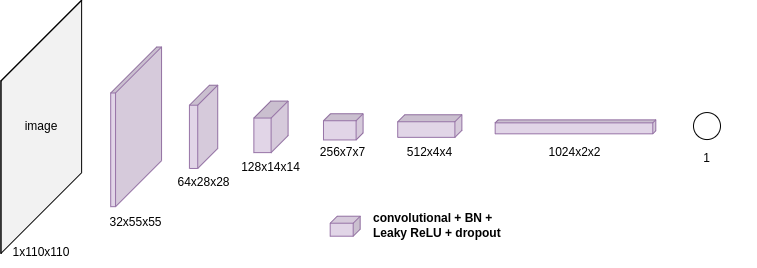
\includegraphics[width=140mm]{img/discriminator.drawio.png}
\caption{CNN architecture of the discriminator.}
\label{img:methods:losses:adversarial}
\end{figure}

To further improve the quality of the generated images, we use discriminator loss together with MSSSIM loss during training. The discriminator loss encourages the generated images to be indistinguishable from real images, while the MSSSIM forces the network to learn features that are based on the cortical activity. We selected a weights of $0.8$ for the discriminator loss and $0.2$ for the MSSSIM loss to balance the two objectives.




% ==================================================
\section{Implementation Details}
\label{methods:implementation-details}
To implement the methods, we used several Python libraries, which are available for both training the models and image augmentation or loss computation.

The linear regression models were trained using Python library scikit-learn\footnote{\url{https://scikit-learn.org}}, specifically using the class LinearRegression\footnote{\url{https://scikit-learn.org/stable/modules/generated/sklearn.linear_model.LinearRegression.html}}.

We implemented and trained the CNN models in the PyTorch\footnote{\url{https://pytorch.org}} framework. The settings for the training were selected as $0.0002$ for the learning rate, batch size of $64$, and the optimization was done using Adam optimizer~\citep{kingma2014adam}\footnote{PyTorch implementation is documented at \url{https://pytorch.org/docs/stable/generated/torch.optim.Adam.html}.} The number of epochs was $15$ (the best model was usually found after training the third epoch) and we used a cosine decay scheduler~\citep{loshchilov2016sgdr}, which starts at the given learning rate and follows the cosine function until it reaches zero learning rate.

For the computation of the loss functions, we used L1Loss and MSELoss implemented by PyTorch\footnote{\url{https://pytorch.org/docs/stable/generated/torch.nn.L1Loss.html} and \url{https://pytorch.org/docs/stable/generated/torch.nn.MSELoss.html}} and SSIMLoss and MS\_SSIMLoss implementations by popular Kornia\footnote{Kornia library is available at \url{https://kornia.github.io}.} library\footnote{\url{https://kornia.readthedocs.io/en/latest/_modules/kornia/losses/ssim.html} and \url{https://kornia.readthedocs.io/en/latest/_modules/kornia/losses/ms_ssim.html}}. All the other loss functions are either implemented in PyTorch or are combinations of these loss functions. The big advantage of these functions is that all of them can be run on GPU, which provides a speedup for their computation.
Note that the losses used for evaluation are computed only for the central 64x64 pixel area, as the reconstruction on the boundaries was not possible by any model we tried. The training loss was always computed for the whole image.
